% Provenance (never printed): see sources/outline_sources.md and sources/book1/BRIEFS.md (g8/05).
\chapter{How the Internet Works}\label{ch:g8:how-the-internet-works}

Sami takes a photo of a fox in the garden and sends it to his cousin on the
other side of the world. Moments later, she sees it. On the way,
the photo was cut into about two thousand pieces, which did not all travel
the same way, passed through many machines that had never heard of Sami,
and were put back together in the right order. This chapter follows those
pieces.

\begin{recall}
A \omterm{def:g5:networks-first-look:network}{network} joins \omterm{def:g1:what-is-a-computer:computer}{computers} so that they can exchange data; the \omterm{def:g5:networks-first-look:internet}{Internet} joins
\omterm{def:g5:networks-first-look:network}{networks} across the world; a \omterm{def:g5:networks-first-look:server}{server} keeps pages and sends them to the
\omterm{def:g5:networks-first-look:page}{browsers} that ask; a \omterm{def:g5:networks-first-look:address}{web address} names a \omterm{def:g5:networks-first-look:server}{server} and a \omterm{def:g3:files-and-folders:file}{file}
(\cref{ch:g5:networks-first-look}). A \omterm{def:g4:memory-and-storage:byte}{byte} is 8 \omterm{def:g5:bits-and-bytes:bit}{bits}, and holds a number from
0 to 255; $n$ \omterm{def:g5:bits-and-bytes:bit}{bits} make $2^n$ patterns (\cref{ch:g8:binary-and-hexadecimal}).
A \omterm{def:g8:dictionaries:dictionary}{dictionary} gives the \omterm{def:g6:variables-and-input:value}{value} of a key (\cref{ch:g8:dictionaries}).
\end{recall}

\section{Messages cut into packets}

\begin{definition}[Packet, packet header]\label{def:g8:how-the-internet-works:packet}
A \emph{packet}\index{packet} is a small piece of the data sent over a
\omterm{def:g5:networks-first-look:network}{network}, with a \emph{packet header}\index{packet header}: a few \omterm{def:g4:memory-and-storage:byte}{bytes} in
front that say where the packet comes from, where it goes, and which piece it
is.
\end{definition}

A \omterm{def:g5:networks-first-look:network}{network} never sends a big \omterm{def:g3:files-and-folders:file}{file} in one go. It cuts it into \omterm{def:g8:how-the-internet-works:packet}{packets} that
travel one by one, each on its own, like the pages of a long letter posted in
separate envelopes. The machine that receives them puts the pieces back in the
order of their numbers. The \omterm{def:g4:programs-and-operating-system:program}{program} below does the same with a short message,
with \omterm{def:g8:how-the-internet-works:packet}{packets} of 6 \omterm{def:g7:strings:string}{characters}; the \omterm{def:g8:how-the-internet-works:packet}{packets} arrive in a mixed order, fixed in
the \omterm{def:g4:programs-and-operating-system:program}{program}.

\omcode{code/grade-8/05-how-the-internet-works/listings/packets.py}{1}{30}{Cutting
a message into \omterm{def:g8:how-the-internet-works:packet}{packets}, then rebuilding it.}\label{lst:g8:how-the-internet-works:packets}

\Needspace*{11\baselineskip}
\omoutput{code/grade-8/05-how-the-internet-works/outputs/packets.txt}{The \omterm{def:g8:how-the-internet-works:packet}{packets}
arrive out of order; their numbers put them
back.}\label{out:g8:how-the-internet-works:packets}

\begin{omfigure}
\begin{tikzpicture}[x=1cm, y=1cm, font=\scriptsize]
  \draw[black!60, fill=ocYellow!20] (0,0) rectangle (2.2,2.4);
  \foreach \y in {0.6,1.2,1.8} { \draw[dashed, black!50] (0,\y) -- (2.2,\y); }
  \foreach \n/\y in {0/2.1, 1/1.5, 2/0.9, 3/0.3} { \node[black!60] at (1.1,\y) {piece \n}; }
  \node[anchor=south] at (1.1,2.5) {the photo};
  \foreach \n/\y in {0/1.4, 1/1.0, 2/0.6, 3/0.2} {
    \draw[black!60, fill=ocInk!80] (3.2,\y*1.6-0.2) rectangle ++(0.5,0.4);
    \node[white] at (3.45,\y*1.6) {\n};
    \draw[black!60, fill=ocYellow!20] (3.7,\y*1.6-0.2) rectangle ++(0.9,0.4);
  }
  \draw[-{Stealth[length=2mm]}, thick] (2.4,1.2) -- (3.0,1.2);
  \node[anchor=south, font=\tiny] at (3.45,2.5) {header};
  \node[anchor=south, font=\tiny] at (4.15,2.5) {data};
  \draw[-{Stealth[length=2mm]}, thick, ocBlue] (4.8,1.2) -- node[above, align=center] {separate\\ paths} (6.4,1.2);
  \foreach \n/\y in {2/1.4, 0/1.0, 3/0.6, 1/0.2} {
    \draw[black!60, fill=ocInk!80] (6.6,\y*1.6-0.2) rectangle ++(0.5,0.4);
    \node[white] at (6.85,\y*1.6) {\n};
    \draw[black!60, fill=ocYellow!20] (7.1,\y*1.6-0.2) rectangle ++(0.9,0.4);
  }
  \node[anchor=south] at (7.3,2.5) {arrival order};
  \draw[-{Stealth[length=2mm]}, thick] (8.2,1.2) -- node[above] {sort} (9.0,1.2);
  \draw[black!60, fill=ocYellow!20] (9.2,0) rectangle (11.4,2.4);
  \node[align=center] at (10.3,1.2) {the photo,\\ rebuilt};
\end{tikzpicture}

{\small A photo cut into numbered \omterm{def:g8:how-the-internet-works:packet}{packets}, each with a small header in front
of its data; they arrive in another order, and their numbers put them back.}
\end{omfigure}

What if a \omterm{def:g8:how-the-internet-works:packet}{packet} is lost on the way? The rebuilt message has a hole:

\omcode{code/grade-8/05-how-the-internet-works/listings/lost_packet.py}{1}{12}{One
\omterm{def:g8:how-the-internet-works:packet}{packet} never arrives.}\label{lst:g8:how-the-internet-works:lost}

\Needspace*{5\baselineskip}
\omoutput{code/grade-8/05-how-the-internet-works/outputs/lost_packet.txt}{A hole
where \omterm{def:g8:how-the-internet-works:packet}{packet} 1 should be.}\label{out:g8:how-the-internet-works:lost}

The receiving machine sees which number is missing and asks for that \omterm{def:g8:how-the-internet-works:packet}{packet}
again. Only the lost piece is sent twice, not the whole photo: that is one
reason for cutting it up.

\section{An address for every machine}

\begin{definition}[IP address]\label{def:g8:how-the-internet-works:ip-address}
An \emph{IP address}\index{IP address} is the number that identifies a
machine on the \omterm{def:g5:networks-first-look:internet}{Internet}. In its common form it is four \omterm{def:g4:memory-and-storage:byte}{bytes}, written as four
numbers from 0 to 255 separated by dots, such as \code{192.168.1.20}.
\end{definition}

% ledger: g8:ipv4-32bits
Four \omterm{def:g4:memory-and-storage:byte}{bytes} are 32 \omterm{def:g5:bits-and-bytes:bit}{bits}. The \omterm{def:g4:programs-and-operating-system:program}{program} cuts an address at its dots and writes
each part in \omterm{def:g5:bits-and-bytes:binary}{binary} on 8 digits, with the \omterm{def:g7:strings:string}{f-string} layout \code{08b}: \code{b}
for \omterm{def:g5:bits-and-bytes:binary}{binary}, \code{08} for 8 digits with zeros in front.

\Needspace*{11\baselineskip}
\omcode{code/grade-8/05-how-the-internet-works/listings/ip_bytes.py}{1}{8}{An \omterm{def:g8:how-the-internet-works:ip-address}{IP
address} as four \omterm{def:g4:memory-and-storage:byte}{bytes}.}\label{lst:g8:how-the-internet-works:ip}

\Needspace*{9\baselineskip}
\omoutput{code/grade-8/05-how-the-internet-works/outputs/ip_bytes.txt}{32
\omterm{def:g5:bits-and-bytes:bit}{bits}.}\label{out:g8:how-the-internet-works:ip}

\begin{omfigure}
\begin{bytefield}[bitwidth=1.15em]{32}
  \bitheader[endianness=big]{0,7,8,15,16,23,24,31} \\
  \bitbox{8}{\code{11000000} = 192} & \bitbox{8}{\code{10101000} = 168} & \bitbox{8}{\code{00000001} = 1} & \bitbox{8}{\code{00010100} = 20}
\end{bytefield}

{\small The address \code{192.168.1.20} as 32 \omterm{def:g5:bits-and-bytes:bit}{bits}: four \omterm{def:g4:memory-and-storage:byte}{bytes}, each written
in decimal between the dots.}
\end{omfigure}

How many such addresses exist? $2^{32}$:

\Needspace*{6\baselineskip}
\omcode{code/grade-8/05-how-the-internet-works/listings/count_addresses.py}{1}{3}{Counting
the addresses.}\label{lst:g8:how-the-internet-works:count}

\Needspace*{7\baselineskip}
\omoutput{code/grade-8/05-how-the-internet-works/outputs/count_addresses.txt}{Fewer
\omterm{def:g4:memory-and-storage:byte}{four-byte} addresses than people.}\label{out:g8:how-the-internet-works:count}

% ledger: g8:ipv6-128bits
About 4.3 billion addresses are fewer than the people on Earth, and many
people own several machines. The newer addresses therefore use 16 \omterm{def:g4:memory-and-storage:byte}{bytes}, 128
\omterm{def:g5:bits-and-bytes:bit}{bits}: $2^{128}$ is a number of 39 digits, enough for every grain of sand many
times over. Both kinds are in use today.

\begin{definition}[Network interface]\label{def:g8:how-the-internet-works:interface}
A \emph{network interface}\index{network interface} is the part of a machine
that connects it to a \omterm{def:g5:networks-first-look:network}{network}: a socket for a cable, or a radio for wi-fi.
A machine has an address for each of its \omterm{def:g5:networks-first-look:network}{network} interfaces.
\end{definition}

\begin{definition}[Network switch]\label{def:g8:how-the-internet-works:switch}
A \emph{network switch}\index{network switch} is a box with many sockets that
joins the machines of one local \omterm{def:g5:networks-first-look:network}{network}, such as those of a home, a school or
an office, and passes each \omterm{def:g8:how-the-internet-works:packet}{packet} to the machine it is for.
\end{definition}

\begin{omfigure}
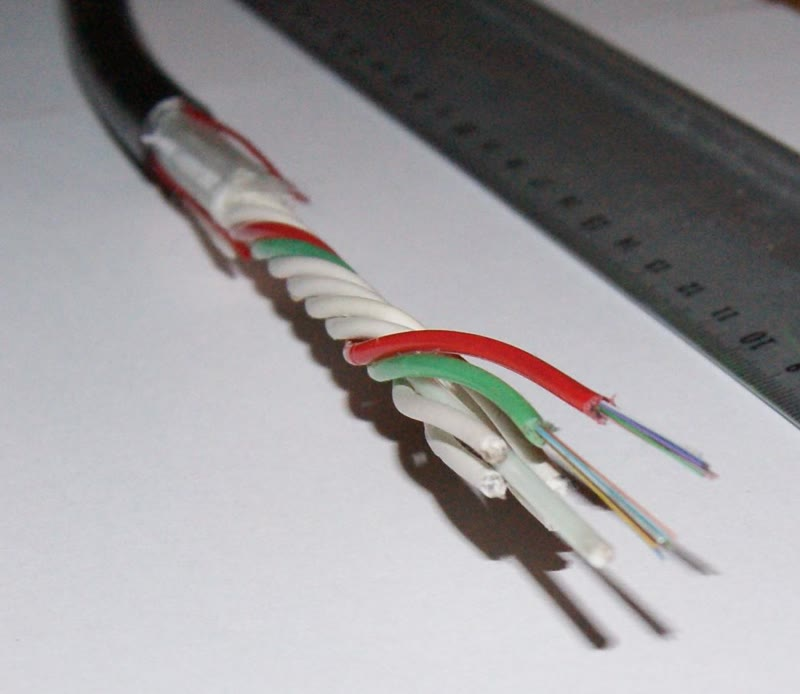
\includegraphics[width=0.45\linewidth]{images/book1/g8-optical-fibre-cable.jpg}

{\small An optical fibre cable made to be buried in the ground, opened: the red
and the green tube each hold 12 coloured glass fibres, each one carrying its
own flashes of light.}
\end{omfigure}

At home, the box from the \omterm{def:g5:networks-first-look:internet}{Internet} provider usually contains a small switch
and a wi-fi radio: the laptop, the phone and the printer of the house are on
one local \omterm{def:g5:networks-first-look:network}{network}. Over long distances, the \omterm{def:g8:how-the-internet-works:packet}{packets} travel as flashes of
light in optical fibres, glass threads thinner than a hair.

\section{Routers}

\begin{definition}[Router]\label{def:g8:how-the-internet-works:router}
A \emph{router}\index{router} is a machine that joins \omterm{def:g5:networks-first-look:network}{networks}. For each
\omterm{def:g8:how-the-internet-works:packet}{packet} it receives, it reads the destination address in the header and passes
the \omterm{def:g8:how-the-internet-works:packet}{packet} one step closer to it, to the next router or to the local \omterm{def:g5:networks-first-look:network}{network}
of the destination.
\end{definition}

No \omterm{def:g8:how-the-internet-works:router}{router} knows the whole \omterm{def:g5:networks-first-look:internet}{Internet}. Each one keeps a table of directions:
``for these addresses, pass to that neighbour''. The \omterm{def:g8:how-the-internet-works:packet}{packet} hops from \omterm{def:g8:how-the-internet-works:router}{router}
to \omterm{def:g8:how-the-internet-works:router}{router}, each choosing only the next step. The \omterm{def:g4:programs-and-operating-system:program}{program} below uses a toy
\omterm{def:g5:networks-first-look:network}{network} of six \omterm{def:g8:how-the-internet-works:router}{routers}, A to F, with a \omterm{def:g8:dictionaries:dictionary}{dictionary} that gives each \omterm{def:g8:how-the-internet-works:router}{router}'s
next step towards F.

\Needspace*{12\baselineskip}
\omcode{code/grade-8/05-how-the-internet-works/listings/path.py}{1}{9}{The path of
a \omterm{def:g8:how-the-internet-works:packet}{packet}, one step at a time.}\label{lst:g8:how-the-internet-works:path}

\Needspace*{5\baselineskip}
\omoutput{code/grade-8/05-how-the-internet-works/outputs/path.txt}{Three
hops.}\label{out:g8:how-the-internet-works:path}

\begin{omfigure}
\begin{tikzpicture}[font=\scriptsize,
    dev/.style={draw=black!60, fill=white, rounded corners=1pt, minimum width=1.0cm, minimum height=0.45cm},
    sw/.style={draw=black!60, fill=ocBlue!20, minimum width=1.2cm, minimum height=0.4cm},
    rt/.style={circle, draw=black!60, fill=ocYellow!40, minimum size=0.6cm, inner sep=0pt}]
  \node[dev] (l1) at (0,1.2) {laptop};
  \node[dev] (p1) at (0,0.4) {phone};
  \node[dev] (q1) at (0,-0.4) {printer};
  \node[sw] (s1) at (1.9,0.4) {switch};
  \foreach \d in {l1,p1,q1} { \draw (\d.east) -- (s1.west); }
  \node[rt] (A) at (3.4,0.4) {A};
  \draw (s1) -- (A);
  \node[rt] (B) at (4.6,1.3) {B};
  \node[rt] (D) at (4.6,-0.5) {D};
  \node[rt] (C) at (5.9,1.3) {C};
  \node[rt] (E) at (5.9,-0.5) {E};
  \node[rt] (F) at (7.2,0.4) {F};
  \foreach \a/\b in {A/B, A/D, B/C, B/D, C/E, D/E, C/F, E/F} { \draw[black!50] (\a) -- (\b); }
  \draw[ocRed, very thick, -{Stealth[length=2mm]}] (A) -- (B);
  \draw[ocRed, very thick, -{Stealth[length=2mm]}] (B) -- (C);
  \draw[ocRed, very thick, -{Stealth[length=2mm]}] (C) -- (F);
  \node[sw] (s2) at (8.7,0.4) {switch};
  \draw (F) -- (s2);
  \node[dev] (l2) at (10.4,0.9) {laptop};
  \node[dev] (sv) at (10.4,-0.1) {server};
  \foreach \d in {l2,sv} { \draw (\d.west) -- (s2.east); }
  \draw[black!40, dashed, rounded corners] (-0.7,-0.8) rectangle (2.6,1.6);
  \node[anchor=north west, black!60] at (-0.7,-0.85) {a home network};
  \draw[black!40, dashed, rounded corners] (8.0,-0.6) rectangle (11.1,1.4);
  \node[anchor=north west, black!60] at (8.0,-0.65) {another local network};
  \node[black!60] at (5.3,-1.15) {routers of the Internet};
\end{tikzpicture}

{\small Two local \omterm{def:g5:networks-first-look:network}{networks}, each joined by a switch, linked through \omterm{def:g8:how-the-internet-works:router}{routers}.
In red, the path of \cref{lst:g8:how-the-internet-works:path}: A, B, C,
F.}
\end{omfigure}

If a link breaks, the \omterm{def:g8:how-the-internet-works:router}{routers} change their tables, and the next \omterm{def:g8:how-the-internet-works:packet}{packets} go
round the break: the \omterm{def:g8:how-the-internet-works:packet}{packets} of one message may well take different paths.

\begin{history}[The first network of networks]
% ledger: g8:arpanet-1969
The ancestor of the \omterm{def:g5:networks-first-look:internet}{Internet}, the ARPANET, was switched on in late October
1969 in the United States. It was the first large \omterm{def:g5:networks-first-look:network}{network} built to connect
different kinds of \omterm{def:g1:what-is-a-computer:computer}{computers} together.
\end{history}

\section{Names turned into addresses}

\begin{definition}[Domain name, domain name system]\label{def:g8:how-the-internet-works:domain-name}
A \emph{domain name}\index{domain name} is a name for a machine on the
\omterm{def:g5:networks-first-look:internet}{Internet}, made of words separated by dots, such as
\code{library.brenmoor.example}. The \emph{domain name system}\index{domain
name system (DNS)} (DNS) is a service, spread over many \omterm{def:g5:networks-first-look:server}{servers}, that answers
the question ``which \omterm{def:g8:how-the-internet-works:ip-address}{IP address} does this name have?''.
\end{definition}

% ledger: g8:dns
People remember names; \omterm{def:g8:how-the-internet-works:router}{routers} need numbers. Before anything else, a \omterm{def:g5:networks-first-look:page}{browser}
asks the name system for the address of the name in the \omterm{def:g5:networks-first-look:address}{web address}. The toy
version is a \omterm{def:g8:dictionaries:dictionary}{dictionary}:

\omcode{code/grade-8/05-how-the-internet-works/listings/names.py}{1}{14}{A toy name
table.}\label{lst:g8:how-the-internet-works:names}

\Needspace*{6\baselineskip}
\omoutput{code/grade-8/05-how-the-internet-works/outputs/names.txt}{An unknown name
has no address.}\label{out:g8:how-the-internet-works:names}

The names ending in \code{.example} and the addresses starting with
\code{192.0.2}, \code{198.51.100} and \code{203.0.113} are kept for examples in
books like this one: they belong to no real machine.

\section{From typing an address to seeing the page}

\begin{definition}[Client]\label{def:g8:how-the-internet-works:client}
A \emph{client}\index{client} is a \omterm{def:g4:programs-and-operating-system:program}{program} that asks a \omterm{def:g5:networks-first-look:server}{server} for something,
such as a \omterm{def:g5:networks-first-look:page}{browser} asking for a page. The client asks; the \omterm{def:g5:networks-first-look:server}{server} answers.
\end{definition}

\begin{omfigure}
\begin{tikzpicture}[font=\scriptsize, x=1cm, y=0.62cm]
  \foreach \x/\t in {0/browser (client), 4.6/name system, 9.2/server} {
    \node[draw=black!60, fill=ocBlue!15, minimum width=2.4cm] at (\x,0) {\t};
    \draw[black!40] (\x,-0.5) -- (\x,-7.5);
  }
  \draw[-{Stealth[length=2mm]}] (0,-1.6) -- node[above] {address of this name?} (4.6,-1.6);
  \draw[-{Stealth[length=2mm]}] (4.6,-2.8) -- node[above] {\code{203.0.113.7}} (0,-2.8);
  \draw[-{Stealth[length=2mm]}, ocRed] (0,-4.2) -- node[above, pos=0.7] {request: send me the page} (9.2,-4.2);
  \foreach \y in {-5.4,-5.9,-6.4,-6.9} { \draw[-{Stealth[length=1.5mm]}, ocBlue] (9.2,\y) -- (0,\y-0.3); }
  \node[anchor=west, ocBlue] at (9.3,-6.1) {the page, in packets};
  \draw[ocMint!80!black, fill=ocMint!25] (-0.3,-8.9) rectangle (0.3,-7.9);
  \node[anchor=east, align=right] at (-0.4,-8.4) {packets put\\ back in order};
  \node[anchor=west] at (0.4,-8.4) {the page is drawn on the screen};
  \node[anchor=east] at (-1.3,-1.6) {1};
  \node[anchor=east] at (-1.3,-2.8) {2};
  \node[anchor=east] at (-1.3,-4.2) {3};
  \node[anchor=east] at (-1.3,-6.1) {4};
\end{tikzpicture}

{\small From a typed name to a page on the screen: the name system gives the
address, the \omterm{def:g8:how-the-internet-works:client}{client} asks the \omterm{def:g5:networks-first-look:server}{server}, and the page comes back in \omterm{def:g8:how-the-internet-works:packet}{packets}.}
\end{omfigure}

Typing \code{library.brenmoor.example} in the address bar sets off the whole
chain of this chapter: the name becomes an address; the request travels in
\omterm{def:g8:how-the-internet-works:packet}{packets}, through switches and \omterm{def:g8:how-the-internet-works:router}{routers}, to the \omterm{def:g5:networks-first-look:server}{server}; the page comes back in
\omterm{def:g8:how-the-internet-works:packet}{packets}, maybe by other paths; the \omterm{def:g5:networks-first-look:page}{browser} puts them in order and draws the
page. It usually takes less than a second.

\section{Speed and delay}

\begin{definition}[Bit rate]\label{def:g8:how-the-internet-works:bit-rate}
The \emph{bit rate}\index{bit rate} of a connection is the number of \omterm{def:g5:bits-and-bytes:bit}{bits} it
can send each second, in \omterm{def:g5:bits-and-bytes:bit}{bits} per second; a megabit per second (Mbit/s) is a
million of them.
\end{definition}

\begin{definition}[Latency]\label{def:g8:how-the-internet-works:latency}
The \emph{latency}\index{latency} of a connection is the time a \omterm{def:g5:bits-and-bytes:bit}{bit} takes to
reach the other end: the delay before anything arrives, however fast the
\omterm{def:g5:bits-and-bytes:bit}{bits} follow each other after that.
\end{definition}

\omterm{def:g8:how-the-internet-works:bit-rate}{Bit rate} is the width of a pipe, \omterm{def:g8:how-the-internet-works:latency}{latency} its length. Part of the \omterm{def:g8:how-the-internet-works:latency}{latency} is
the travel of the light itself: in a glass fibre, light covers about 200,000
kilometres each second, two thirds of its speed in empty space.

\Needspace*{12\baselineskip}
\omcode{code/grade-8/05-how-the-internet-works/listings/delay.py}{1}{9}{The travel
time over a few distances, and the time to send a
photo.}\label{lst:g8:how-the-internet-works:delay}

\Needspace*{8\baselineskip}
\omoutput{code/grade-8/05-how-the-internet-works/outputs/delay.txt}{One millisecond
(ms) is a thousandth of a second.}\label{out:g8:how-the-internet-works:delay}

Across a town, the light travel is nothing; across half the world, it is a
tenth of a second, and no faster connection can shorten it. Sending the
3 \omterm{def:g4:memory-and-storage:units}{megabytes} of a photo, $3{,}000{,}000 \times 8 = 24$ million \omterm{def:g5:bits-and-bytes:bit}{bits}, at 10
megabits per second takes 2.4 seconds: there, a faster connection helps.

\begin{dated}{2026}
% ledger: g8:broadband-2026
In the United Kingdom, the telecoms regulator reported that the home
connections in use could reach 285 megabits per second on average in 2025,
against 223 in 2024; most homes with optical fibre chose a plan of 300
megabits per second or less. Fast home plans reach 1,000 megabits per second,
a gigabit.

% ledger: g8:datacentres-energy
The data centres that hold the \omterm{def:g5:networks-first-look:server}{servers} of the \omterm{def:g5:networks-first-look:internet}{Internet} used about 415
terawatt-hours of electricity in 2024, about 1.5\,\% of the world's
electricity, according to the International Energy Agency.
\end{dated}

\begin{omfigure}
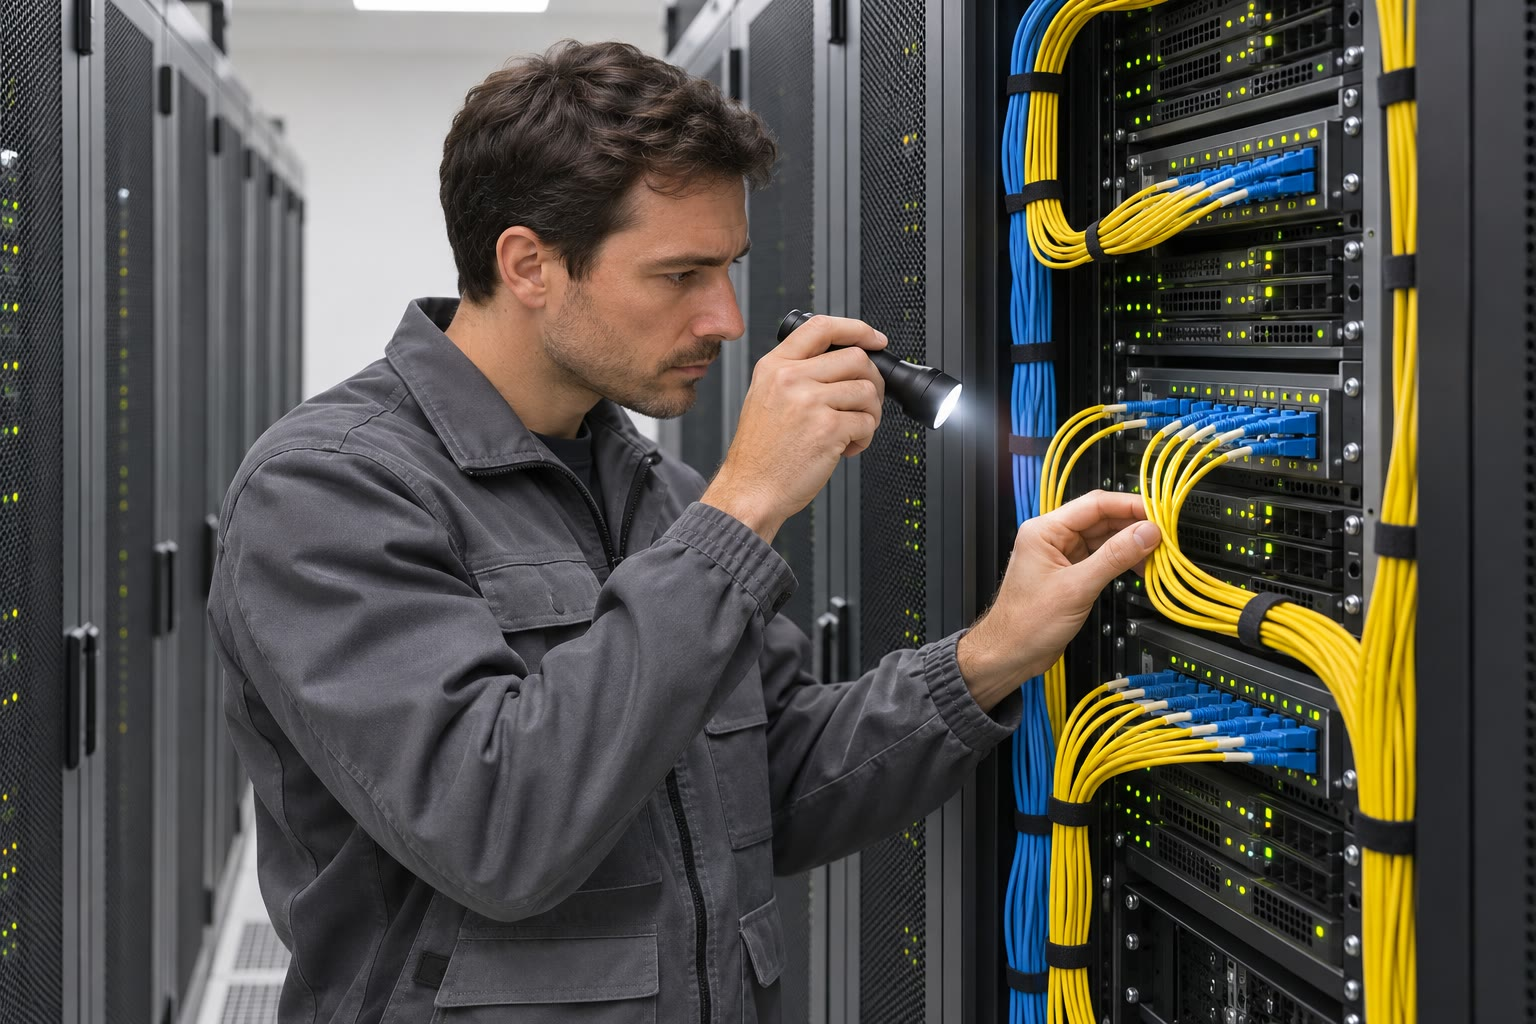
\includegraphics[width=0.55\linewidth]{images/book1/ai/g8-how-the-internet-works-data-centre.jpg}

{\small In a data centre, rows of cabinets hold \omterm{def:g5:networks-first-look:server}{servers}, switches and
\omterm{def:g8:how-the-internet-works:router}{routers}, joined by cables and optical fibres.}
\end{omfigure}

\section{Exercises}

\begin{exercise}[$\star$]\label{exo:g8:how-the-internet-works:1}
What does \cref{lst:g8:how-the-internet-works:ip} print for the address
\code{10.0.0.255}?
\end{exercise}

\begin{exercise}[$\star$]\label{exo:g8:how-the-internet-works:2}
Four \omterm{def:g8:how-the-internet-works:packet}{packets} arrive in this order: (2, \code{"ld"}), (0, \code{"Hel"}),
(3, \code{"!"}), (1, \mbox{\code{"lo wor"}}). What is the rebuilt message?
\end{exercise}

\begin{exercise}[$\star$]\label{exo:g8:how-the-internet-works:3}
What does \cref{lst:g8:how-the-internet-works:path} print if the \omterm{def:g8:how-the-internet-works:packet}{packet}
starts at \omterm{def:g8:how-the-internet-works:router}{router} D?
\end{exercise}

\begin{exercise}[$\star$]\label{exo:g8:how-the-internet-works:4}
Write a \omterm{def:g7:functions:function}{function} \code{cut(text, size)} that cuts a text into pieces of
at most \code{size} \omterm{def:g7:strings:string}{characters}, numbered from 1, each a \omterm{def:g8:dictionaries:dictionary}{dictionary} with the keys
\code{"number"}, \code{"of"} (how many pieces there are in all, so that the
receiver knows when every piece has come) and \code{"data"}.
\end{exercise}

\begin{exercise}[$\star\star$]\label{exo:g8:how-the-internet-works:5}
This rebuild keeps the numbers as text. With 12 \omterm{def:g8:how-the-internet-works:packet}{packets} of one letter, from
\code{"a"} to \code{"l"}, it returns \code{"abklcdefghij"}. Why? Fix it.

\omcode{code/grade-8/05-how-the-internet-works/exercises/rebuild_bug.py}{1}{8}{A
rebuild with numbers as text.}\label{lst:g8:how-the-internet-works:rebuild-bug}
\end{exercise}

\begin{exercise}[$\star\star$]\label{exo:g8:how-the-internet-works:6}
This \omterm{def:g7:functions:function}{function} accepts \code{"192.168.300.1"}. (\code{isdigit()} is true when
a \omterm{def:g7:strings:string}{string} is made of digits only.) What is wrong with that address? Add the
missing check.

\omcode{code/grade-8/05-how-the-internet-works/exercises/valid_bug.py}{1}{9}{A check
that misses something.}\label{lst:g8:how-the-internet-works:valid-bug}
\end{exercise}

\begin{exercise}[$\star\star$]\label{exo:g8:how-the-internet-works:7}
In many homes, the machines of the local \omterm{def:g5:networks-first-look:network}{network} share the first three \omterm{def:g4:memory-and-storage:byte}{bytes}
of their addresses. Write a \omterm{def:g7:functions:function}{function} \code{same_network(a, b)} that tells
whether two addresses do.
\end{exercise}

\begin{exercise}[$\star\star$]\label{exo:g8:how-the-internet-works:8}
Write a \omterm{def:g7:functions:function}{function} \code{sending_time(size_bytes, rate)} that returns the time,
in seconds, to send a \omterm{def:g3:files-and-folders:file}{file} of \code{size_bytes} \omterm{def:g4:memory-and-storage:byte}{bytes} at \code{rate} \omterm{def:g5:bits-and-bytes:bit}{bits} per
second. How long does a 5-megabyte \omterm{def:g3:files-and-folders:file}{file} take at 20 megabits per second?
\end{exercise}

\begin{exercise}[$\star\star$]\label{exo:g8:how-the-internet-works:9}
How many different addresses of four \omterm{def:g4:memory-and-storage:byte}{bytes} are there? Write the number in
full.
\end{exercise}

\begin{exercise}[$\star\star\star$]\label{exo:g8:how-the-internet-works:10}
How long does light take to cross 6,000 kilometres of glass fibre, in
milliseconds? Use the speed of the weekend problem's \omterm{def:g4:programs-and-operating-system:program}{program}.
\end{exercise}

\begin{exercise}[$\star\star\star$]\label{exo:g8:how-the-internet-works:11}
A \omterm{def:g3:files-and-folders:file}{file} of 1,000,000 \omterm{def:g4:memory-and-storage:byte}{bytes} is sent in \omterm{def:g8:how-the-internet-works:packet}{packets} of 1,500 \omterm{def:g4:memory-and-storage:byte}{bytes}, 40 of which are
header. How many \omterm{def:g8:how-the-internet-works:packet}{packets} are needed, and how many \omterm{def:g4:memory-and-storage:byte}{bytes} are sent in all?
\end{exercise}

\begin{exercise}[$\star\star\star$]\label{exo:g8:how-the-internet-works:12}
\omterm{def:g8:how-the-internet-works:packet}{Packets} may arrive twice. Write a \omterm{def:g7:functions:function}{function} \code{reassemble(packets, count)}
that rebuilds a message of \code{count} \omterm{def:g8:how-the-internet-works:packet}{packets}, keeps one copy of each
number, and also returns the \omterm{def:g7:lists:list}{list} of the numbers that are missing.
\end{exercise}

\section{Problem: A Photo to the Other Side of the World}

\begin{problem}[{Weekend problem --- a photo to the other side of the world}]\label{pb:g8:how-the-internet-works:1}
Sami's photo weighs 3 \omterm{def:g4:memory-and-storage:units}{megabytes}, 3,000,000 \omterm{def:g4:memory-and-storage:byte}{bytes}. It goes to his cousin
20,000 kilometres away, half way round the Earth.

\needspace{4\baselineskip}\medskip\noindent\textbf{Part I --- Packets.}
% ledger: g8:packet-1500
% ledger: g8:headers-40
A \omterm{def:g8:how-the-internet-works:packet}{packet} on most \omterm{def:g5:networks-first-look:network}{networks} holds at most 1,500 \omterm{def:g4:memory-and-storage:byte}{bytes}, and at least 40 of them
are headers: 20 for the address part and 20 for the part that numbers the
pieces.
\begin{enumerate}
  \item How many \omterm{def:g4:memory-and-storage:byte}{bytes} of the photo fit in one \omterm{def:g8:how-the-internet-works:packet}{packet}?
  \item How many \omterm{def:g8:how-the-internet-works:packet}{packets} does the photo need? Is the last one full?
  \item How many \omterm{def:g4:memory-and-storage:byte}{bytes} of header are sent, and what fraction of the whole is
    that?
\end{enumerate}

\needspace{4\baselineskip}\medskip\noindent\textbf{Part II --- The program.}
% ledger: g8:fibre-index
For the speed of light in a fibre, the \omterm{def:g4:programs-and-operating-system:program}{program} uses a figure from a fibre
maker's data sheet: light in its fibre is 1.468 times slower than in empty
space, where it covers 300,000 kilometres per second.

\omcode{code/grade-8/05-how-the-internet-works/listings/photo_trip.py}{1}{19}{The
trip of the photo.}\label{lst:g8:how-the-internet-works:photo}

\begin{enumerate}[resume]
  \item What do lines 6 to 8 compute, and why the \code{if}?
  \item Run the \omterm{def:g4:programs-and-operating-system:program}{program}. What is the propagation time over 20,000 kilometres?
  \item What is the sending time at 10 megabits per second? At 100?
  \item Why does the sending time use \code{total}, not \code{photo}?
\end{enumerate}

\needspace{4\baselineskip}\medskip\noindent\textbf{Part III --- What matters.}
\begin{enumerate}[resume]
  \item At 10 megabits per second, which part of the time is larger, sending
    or propagation?
  \item What does a ten times faster connection change, from 10 to 100
    megabits per second? And from 100 to 1,000?
  \item Can any connection bring the photo in less than 0.098 seconds? Why?
  \item The \omterm{def:g8:how-the-internet-works:router}{routers} on the way add a little delay each. Does that change the
    answer to the previous question?
  \item State the result.
\end{enumerate}
\end{problem}
